CEBAF (Fig.\ref{Figure:cebaf}) generates the electron beam used in the HPS experiment. CEBAF is an accelerator characterized by its nearly continuous duty cycle and ability to provide electron beams to multiple experimental halls simultaneously. The CEBAF accelerator is a recirculating linac in the shape of a racetrack through which electron beam bunches can pass multiple times, boosted in energy with each pass, before being delivered to a specific hall. 

\begin{figure}[H]
  \centering
      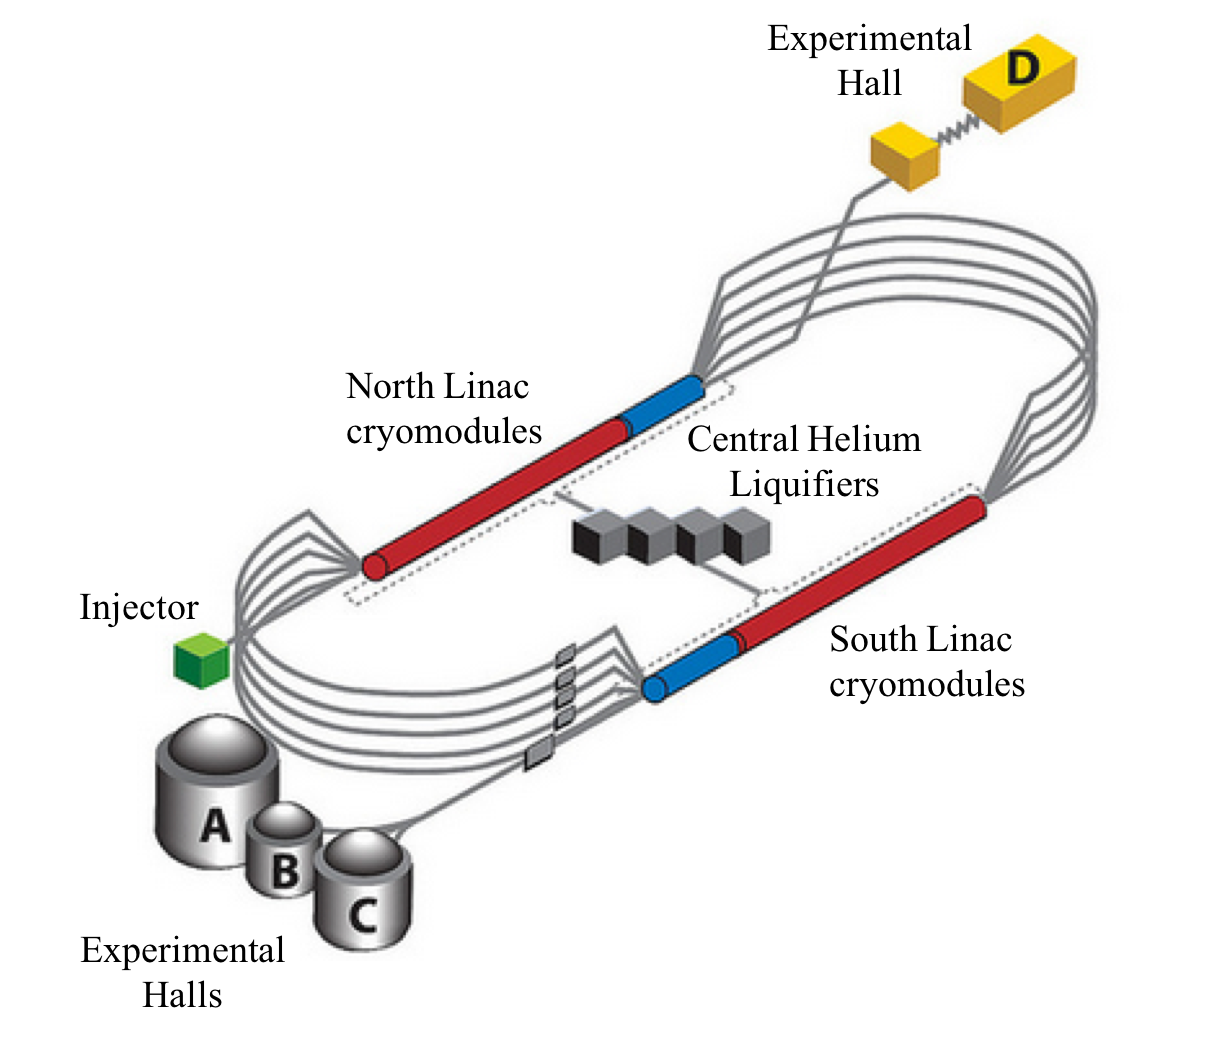
\includegraphics[width=0.75\textwidth]{pics/experiment/cebafLabel.png}
  \caption[CEBAF accelerator]{The CEBAF accelerator was upgraded prior to the HPS experiment to include additional cryomodules and central helium liquifier (CHL) for higher energy, a fifth pass, and a fourth experimental hall.}
  \label{Figure:cebaf}
\end{figure}

The injector energy is 100~MeV, designed for a maximum of five passes (upgraded from four passes) with an energy per pass of 2.2~GeV (upgraded from 1.1~GeV). These upgrades double the maximum energy output of the accelerator. While the accelerator frequency operates at 1500~MHz, a new 750~MHz RF separator was installed in order to provide beam to all four halls simultaneously. With these upgrades, the halls can receive the beam at 250 or 500~MHz and operate at different energies \cite{kazimi}. 

HPS is the first experiment to run in Hall B after the accelerator was upgraded. After a problem occurred in one CHL during the Engineering Run in the spring of 2015, HPS obtained dedicated beam time as one of the few experiments that could continue to take physics data with the accelerator operating at a single pass using the remaining CHL. The resulting energy for the Engineering Run, 1.05~GeV, would have been impossible to obtain with the simultaneous running of other experiments requiring 2.2~GeV per pass.  
